\chapter{Inledning} 
%Denna första del fungerar som bekgrund, men behöver ingen rubrik tycker jag. Hamnar direkt under rubriken Inledning.
%Denna första del fungerar som bekgrund, men behöver ingen rubrik tycker jag. Hamnar direkt under rubriken Inledning.
Robothänder kan användas som ett mycket effektivt hjälpmedel, inte bara för personer i behov av en protes, utan även i industriella tillämpningar. Monotona, fysiskt tunga, och direkt farliga arbeten kan utföras av en robothand istället för en människa. I industritillämpningar kan robothänder vara förprogrammerade att utföra specifika uppgifter vilket inte kräver manuell styrning medan en protes kan styras med ett neuralt gränssnitt. Att manuellt kunna fjärrstyra robothänder har gett upphov till flera användningsområden. Möjligheten att finkänsligt kunna manipulera objekt utan att finnas på samma plats som objektet är användbart inom flera områden.

En utmaning med att fjärrstyra en robothand är att få styrningen att kännas intuitiv. En möjlig lösning är att styrningen sker med en handske, så att robothanden efterliknar användarens rörelser för att det ska kännas mer intuitivt. Detta förutsätter att robothanden har människoliknande rörelsemöjligheter. I rapporten "Human Grasp Choice And Robotic Grasp Analysis" redogörs det för vilka olika typer av grepp den mänskliga handen kan utföra och hur komplext det är att efterlikna dessa med en robothand. Greppbilderna presenteras i ett schema, se appendix "Cutkoskys grepphierarki" (Cutkosky och Howe, 1990). Cutkosky och Howe nämner i reflektioner av sina undersökningar att designen av en robothand ska utgå ifrån vilka grepp den ska kunna utföra och om den designas efter att kunna hantera ett specifikt föremål är det snarare ett greppverktyg än en hand. 

Ytterliggare en utmaning är att undvika att skada eller felhantera föremålet med robothanden då användaren inte själv kan känna hur hårt den greppar. Det pågår idag mycket forskning och utveckling av robothänder och detta har resulterat i mycket avancerade prototyper.  En av de mest avancerade just nu inom genren som styrs med hjälp av en handske är Festo's ExoHand (Festo,2012). Med åtta dubbelverkande pneumatiska aktuatorer och 16 trycksensorer kan den noga efterlikna användarens rörelse och dessutom ge haptisk återkoppling som möjliggör för användaren att noga reglera greppkraften. (Skriv om force/velocity control handen! för att det är ett annat problematiskt sätt att lösa greppning av objekt.)En annan metod som utvecklats för att varsamt kunna hantera objekt med robothandprotes är force/velocity...

Stora hinder i utvecklingen av robothänder generellt har varit de höga kostnaderna, eftersom den mänskliga komplexa fingerfärdigheten och styrningen ställer höga krav på komponenter (ref 2). Kostnaden för en hand som kan efterlikna den mänskliga handens rörelser överstiger ofta 10 000 dollar (ref längst ner). Kostnaden stiger i regel med ökat antal kontrollerbara frihetsgrader och ökad komplexitet. 
 


%Någon ha tagit bort förutsättningarna vi hade. Meccano och pengar t.ex. Victor sa uttryckligen att det ska ingå i inedningen.




\section{Tekniskt bidrag}% "Contributions" -- Syfte.
I denna rapport redogörs för utvecklingen av ett system innehållande en robothand med tre fingrar som fjärrstyrs från en styrhandske. Robothanden designas liknande en mänsklig hand i sina rörelser för att möjliggöra att styrningen blir intuitiv. För att fingrarna ska röra sig flexibelt krävs det att den mekaniska konstruktionen tillåter en rörelse med flera frihetsgrader. För att uppnå detta är handens fingrar konstruerade att aktueras både via genomlöpande senor och stag. Vidare krävs stabila styrsignaler från styrhandsken till robothanden som utnyttjas för att åstadkomma god åtföljning. Detta uppnås genom designade butterworthfilter och programmering där ändrad fingervinkel hos användaren omvandlas till en motsvarande servovinkel. För att användare med olika handstorlek ska uppnå samma resultat är det nödvändigt att kalibrera handsken för varje ny användare. Kalibreringenen sker med hjälp av två knappar som sitter på handskens kretskort.

För att undvika skador på objekt som robothanden hanterar ska ett bibliotek av objekt kunna implementeras i robothandens mikrokontroller som möjliggör objektidentifiering. Varje objekt har ett fördefinierat högsta tryck som robothanden får utsätta den för. Om operatören försöker greppa hårdare än det fördefinierade trycket reglerar robothanden detta för att undvika skada. Objektidentifieringen är baserad på igenkänning av objektets storlek genom att, utifrån vinklar på de styrande servomotorerna, beräkna avståndet mellan de tryckbelastade punkterna på robotfingrarna.

Robothanden följer användarens fingerrörelser tills dess att den greppar ett av flera fördefinerade, kända objekt, då den istället verkar för att hålla objektet med en önskad kraft, tills dess att användaren visar att den vill släppa objektet igen genom att öppna sin hand. Nedan visas ett flödesschema för överskådligt beskriva hur robothanden principiellt fungerar.

\begin{figure}[H]
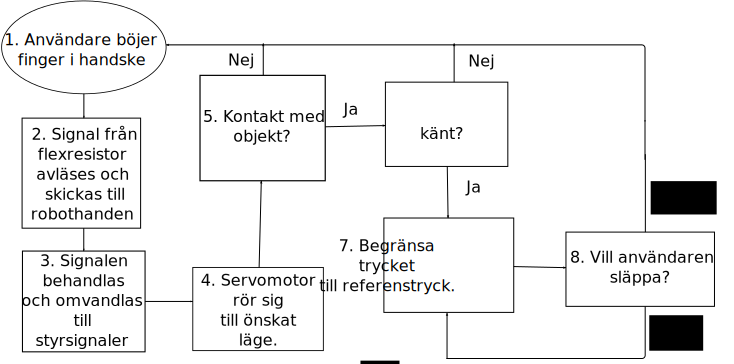
\includegraphics[width=.90\textwidth]{img/flodesschema}
\caption{Flödesschema över en tänkt signals väg genom robothanden.
\comment{det borde inte stå ändringen etc. det är inget som registrerar ``ändringar'' per se, signalen bearbetas kontinuerligt med eller utan ändringar}}
\label{flodesschema}
\end{figure}

\begin{enumerate}
\item Önskat fingerläge ges genom att användaren böjer sitt finger i kontrollhandsken.
\item Flexresistor på kontrollhandsken ändrar resistans.
\item Den ändrade resistansen avläses av en Arduino Micro enhet på kontrollhandsken som skickar den via bluetooth till en Arduino Mega enhet på robothanden.
\item Värdet på resistansen omvandlas till PWM-signal som kalibrerats av användaren vid uppstart.
\item PWM-signaler matas till aktuatorer som ställer sig i önskad vinkel.
\item Feedback från trycksensorer avläses och leder till ett stopp av aktueringen om avläst tryck är högre än fördefinerad gräns.
\end{enumerate}
Robothanden kan delas in i tre delsystem som samverkar för att uppfylla handens funktion. Delsystemen är styrhandske, styrsystem och robothand. Användaren har på sig styrhandsken och styrsystemet verkar för att robothanden ska imitera användarens fingerrörelser tills dess att robothanden kommer i kontakt med ett objekt.



%Detta är just nu en förklaring på vårt systems funktion bara. Bör ingå mer tekniskt? Vilka medel vi använt o så.
\section{Prestanda}

Budgeten för prototypen är 5000 kr vilket begränsar komplexiteten och antal frihetsgrader. Robothanden har därför endast 2 fingrar och en tumme med sammanlagt åtta frihetsgrader varav två är tvångsstyrda. Skelettet till robothanden har byggts i meccano (ref till förklaring av meccano) vilket begränsar designen till standardiserade mått och begränsar stabiliteten i kontruktionen. Robothanden är försedd med tre trycksensorer vilket avsevärt begränsar antal grepp som möjliggör objektidentifiering. 

Efter utförda funktionstester har följande uppgifter verifierats:
\begin{itemize}
\item Gripa och lyfta ett mjölkpaket med en vikt av ett kg. 
\item Gripa och lyfta en mutter av storlek M10 mellan tumme och pekfinger. 
\item Lyfta en last motsvarande ett kg på mitten av två fingrar.
\item Lyfta upp en snusdosa.
\item Kan reglera hur hårt den greppar tre stycken bestämda objekt för att undvika skada. (Se vilka objekt här?)
\item Kan sluta sig till knuten näve från öppen hand på under en sekund.
\end{itemize}
\newpage
\section{Rapportens Upplägg}
%\comment{'' "Report outline" describes very short what is presented in each of the following chapters. From this outline it should be clear which chapters give a theoretical backgrond, which chapter describe tools you use, which describe your contribution, and which describes your results.''-Jonas}

Rapporten är upplagd som följer:\\
I kapitel 2 beskrivs de fysiska komponenterna i systemet. Detta innefattar robothandens mekaniska design, trycksensorer, aktuatorer och kraftöverföring samt styrhandskens utformning. Följande kapitel beskriver principen bakom objektidentifieringen och begränsningen av tryck. I nästa kapitel redogörs för vilka digitaltekniska komponenter som används, det vill säga de två Arduino mikrokontrollerna och bluetooth-enheterna som sköter den trådlösa kommunikationen. I kapitel 5 förklaras hur uppmätta signaler från systemets sensorer samplas, analyseras och filtreras. I kapitel 6 presenteras hur väl objektidentifieringen fungerar i praktiken, samt hur väl handen lyckas begränsa kontakttrycket efter identifiering, tillsammans med demonstationsbilder som visar hur robothanden greppar olika objekt. Den tekniska rapporten avslutas med kapitel 7, där möjliga felkällor diskuteras och framtida förbättringar presenteras.
Viktigt att nämna är att robothanden är framtagen som ett kandidatarbete under begränsad tid med begränsad budget, vilket medfört att avgränsingar införts. Om dessa avgränsningar och andra projektmässiga aspekter kan man läsa efter den tekniska rapporten, det vill säga i kapitel 8.


%Projektdelen borde vara i en avskild del "del 2" t.ex med egna kapitel, efter appendix?

%Kapitel 1 2 3 är upplagd som en teknisk rapport där fokus ligger på utförandet och de verktyg som använts.

%Kapitel 4 och framåt är projektinriktat och fokuserar på hur projektet utfördes


%\section{Avgränsningar} Detta ska smältas ihop med inledning
%Budgeten för prototypen är 5000 kr vilket begränsar komplexiteten och antal frihetsgrader. Robothanden har därför endast 2 fingrar och en tumme med sammanlagt åtta frihetsgrader varav två är tvångsstyrda. Skelettet till robothanden har byggts i meccano (ref till förklaring av meccano) vilket begränsar designen till standardiserade mått och begränsar stabiliteten i kontruktionen. Robothanden är försedd med tre trycksensorer vilket avsevärt begränsar antal grepp som möjliggör objektidentifiering.

 
 



%\section{Vad inledningen ska innehålla enligt anvisningar}
%Inledningen sätter in rapporten i ett sammanhang och visar dess
%relevans och nyhetsvärde. Den fungerar som en introduktion till
%hela rapporten och ska ge läsaren nödvändig information som
%behövs för att ta del av dess innehåll.
%Inledningen innehåller normalt en syftesformulering som ofta
%ställs i relation till en bakgrund eller kort historik. I många fall
%är syftesformuleringen nära relaterad till den
%problemformulering som är viktig för att såväl läsare som
%skribent ska kunna utnyttja rapporten väl. Det bör också stå
%något om undersökningens eller experimentets omfattning och
%anledningar till särskilda avgränsningar. Vidare bör också
%metod finnas med, men endast i syfte att ange vilken typ av
%undersökning som gjorts. Metoden utvecklas i andra avsnitt av
%rapporten.
%Man brukar ange bakgrund, syfte och metod som inledningens
%obligatoriska funktioner. Ibland signaleras även centrala resultat
%redan i inledningen.
%Inledningen är den första sidan som sidnumreras.



%1 http://www.shadowrobot.com/products/dexterous-hand/

%2 http://www.nytimes.com/2013/03/30/science/making-robots-mimic-the-human-hand.html?_r=0

%ExoHand 3 http://www.forbes.com/sites/singularity/2012/07/06/sophisticated-robotic-hand-also-doubles-as-a-human-exoskeleton/

%(Cutkosky och Howe, 1990)
%http://biorobotics.harvard.edu/pubs/1990/human%20grasp%20choice.pdf

%Grepp identifiering. Kan kanske bli användbart vid objektidentifieringssnack http://cg.cis.upenn.edu/hms/research/RIVET/graspTypeRecog.pdf